% Diagram of the pyroprocessing material flow
% Authors: Greg Westphal and Kathryn Huff
\documentclass[border=10pt]{standalone}
\usepackage{tikz}
\usetikzlibrary{arrows.meta}
\tikzset{%
  >={Latex[width=2mm,length=2mm]},
  % Specifications for style of nodes:
            base/.style = {rectangle, rounded corners, draw=black,
                           minimum width=3cm, minimum height=1cm,
                           text centered, font=\sffamily},
       bluebox/.style = {base, fill=gray!15}, %blue!30
       redbox/.style = {base, fill=white!30}, %red
       greenbox/.style = {base, fill=white!30}, %green
       process/.style = {base, minimum width=2.5cm, fill=gray!30, %orange!15
                           font=\ttfamily},
}
% Drawing part, node distance is 1.5 cm and every node
% is prefilled with white background
\begin{document}
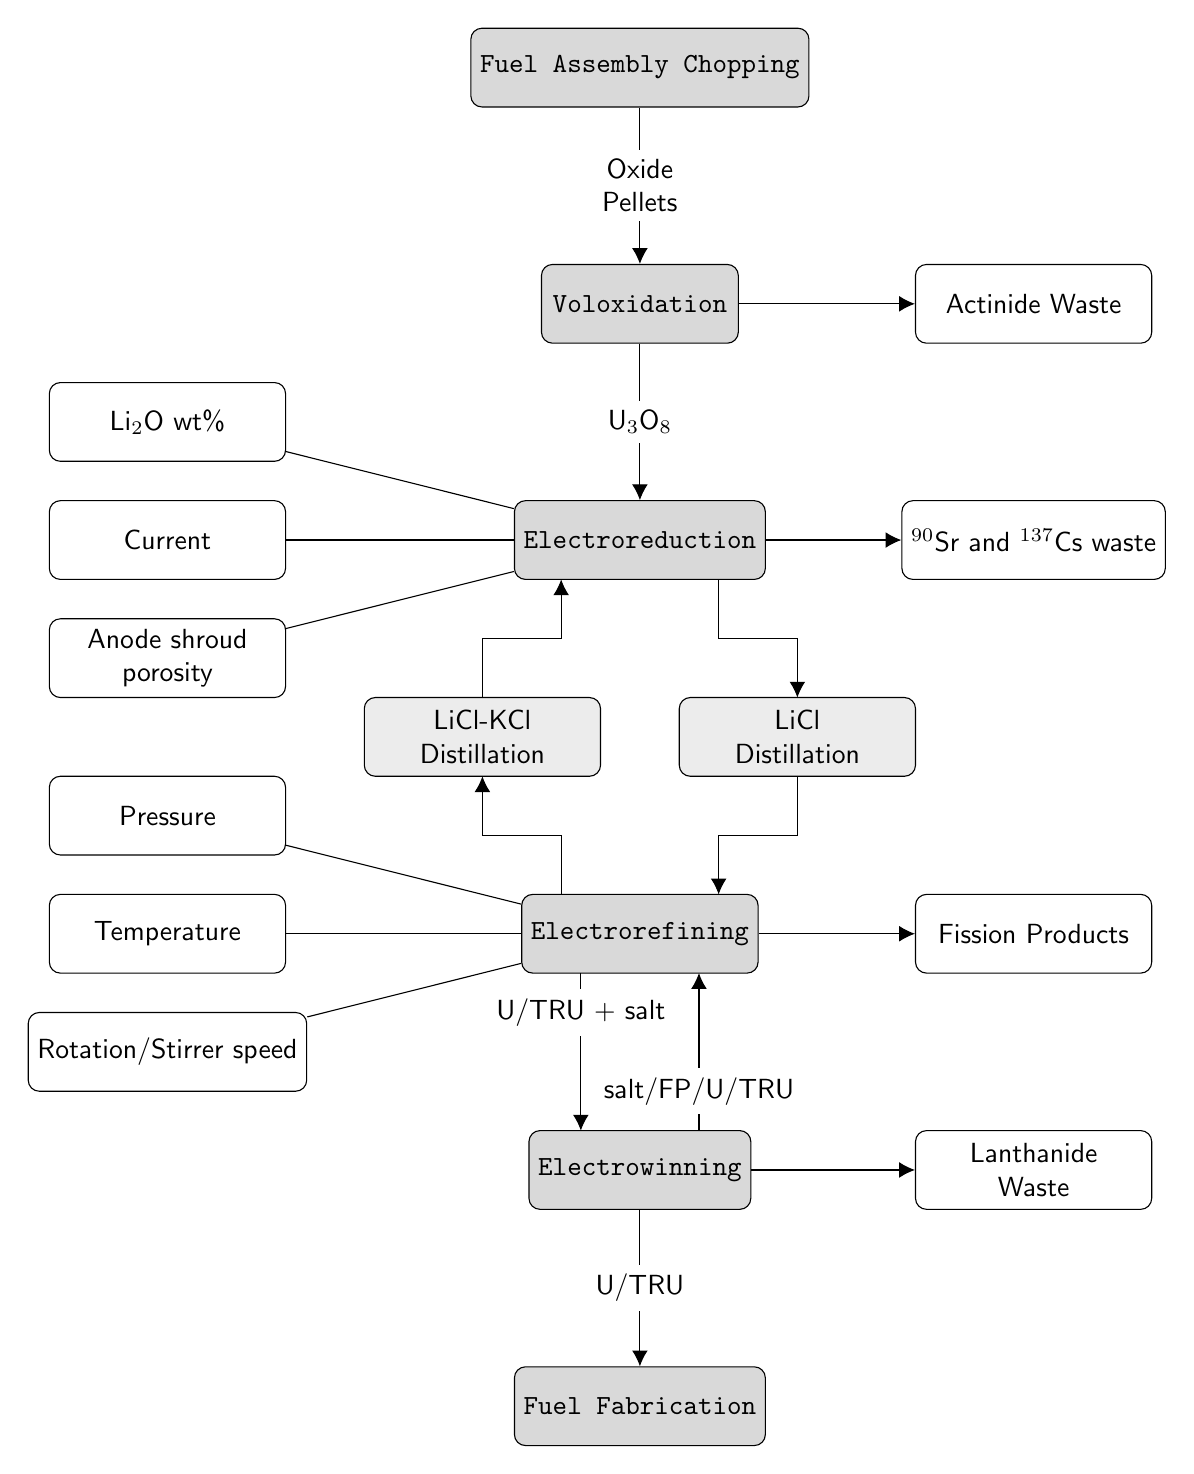
\begin{tikzpicture}[node distance=3cm,
    every node/.style={fill=white, font=\sffamily}, align=center]
  % Specification of nodes (position, etc.)
  
  \node (chop)				[process] {Fuel Assembly Chopping};
  \node (volox)				[process, below of=chop] {Voloxidation};
  \node (reduction)			[process, below of=volox] {Electroreduction};
  \node (actinide)			[redbox, right of=volox, xshift=2cm] {Actinide Waste};
  \node (decay)				[redbox, right of=reduction, xshift=2cm] {$^{90}$Sr and $^{137}$Cs waste};
  \node (refining)			[process, below of=reduction, yshift=-2cm] {Electrorefining};
  %\node (winning)			[process, below of=refining, xshift=3cm] {Electrowinning};
  \node (Li2O)	 			[greenbox, left of=reduction, xshift=-3cm, yshift=1.5cm] {Li$_2$O wt\%};
  \node (temp)	 			[greenbox, left of=refining, xshift=-3cm] {Temperature};
  \node (fission) 			[redbox, right of=refining, xshift=2cm] {Fission Products};
  \node (pressure)			[greenbox, left of=refining, xshift=-3cm, yshift=1.5cm] {Pressure};
  \node (rotation)	 		[greenbox, left of=refining, xshift=-3cm, yshift=-1.5cm] {Rotation/Stirrer speed};
  \node (current)	 		[greenbox, left of=reduction, xshift=-3cm] {Current};
  \node (porosity)			[greenbox, left of=reduction, xshift=-3cm, yshift=-1.5cm] {Anode shroud \\ porosity};
  \node (LiCl)				[bluebox, below of=reduction, xshift=2cm, yshift=0.5cm] {LiCl \\ Distillation};
  \node (LiCl-KCl)			[bluebox, below of=reduction, xshift=-2cm, yshift=0.5cm] {LiCl-KCl \\ Distillation};
  \node (winning)			[process, below of=refining] {Electrowinning};
  %\node (cd distl)			[bluebox, below of=winning] {Cd Distillation};
  \node (lanth)				[redbox, right of=winning, xshift=2cm] {Lanthanide \\ Waste};
  \node (fuel fab) 			[process, below of=winning] {Fuel Fabrication};
  
  \draw[->]					(chop) -- (volox) node[midway] {Oxide \\ Pellets};
  \draw[->]					(volox) -- (reduction) node[midway] {U$_3$O$_8$};
  \draw[->]					(volox) -- (actinide);

  \draw[->]					(reduction) -- (decay);
  \draw[-]					(Li2O) -- (reduction);
  \draw[-]					(porosity) -- (reduction);
  \draw[-]					(current) -- (reduction);
  \draw[-]					(pressure) -- (refining);
  \draw[-]					(temp) -- (refining);
  \draw[-]					(rotation) -- (refining);
  \draw[->]					(refining) -- (fission);
  %\draw[->]					(refining)++(0.75,-0.5) -- ++(0,-1) -- ++(0.75,0) -| (winning);
  \draw[->]					(refining)++(-0.75,-0.5) -- ++(0,-2)(winning) node[near start] {U/TRU + salt};
  \draw[->]					(winning)++(0.75,0.5) -- ++(0,2) (refining) node[near start] {salt/FP/U/TRU};
  %\draw[->]					(winning) -- ++(0,-1.25) -- ++(-2,0)  node[midway] {U} -- (fuel fab);
  \draw[->]					(winning) -- (fuel fab) node[midway] {U/TRU};
  \draw[->]					(reduction)++(1,-0.5) -- ++(0,-0.75) -- ++(1,0) -- ++(0,-0.75) (LiCl);
  \draw[->]					(LiCl) -- ++(0,-1.25) -- ++(-1,0) -- ++(0,-0.75) (refining);
  \draw[->]					(refining)++(-1,0.5) -- ++(0,0.75) -- ++(-1,0) -- ++(0,0.75) (LiCl-KCl);
  \draw[->]					(LiCl-KCl)++(0,0.5) -- ++(0,0.75) -- ++(1,0) -- ++(0,0.75) (reduction);
  \draw[->]					(winning.east) -- (lanth);
  %\draw[->]					(winning) -- (cd distl);
  %\draw[->]					(cd distl) -- (fuel fab) node[midway] {U/TRU};
  \end{tikzpicture}
\end{document}

